\section{Attacks on the Protocol}
\label{sec:insecure-attacks}

The Insecure CC Protocol is vulnerable to a number of attacks that can be performed by an external adversary.
We classify these attacks into four broad categories:
    eavesdropping, skimming attacks, relay attacks, and attacks facilitated by compromised Points of Sale.
In this section, we describe these attacks in detail.


\subsection{Eavesdropping}
\label{sec:insecure-eavesdropper}
The goal of an eavesdropper is to gain the victim's credit card number and expiration date.
Eavesdropping is a passive attack, where the eavesdropper hears all communication between the Point of Sale and the credit card.
(Communication between the Cank and the Point of Sale is securely transmitted over the Internet.)
An outline of this attack is shown in Figure \ref{fig:insecure-eavesdropper}.

\begin{figure}
  \caption{Eavesdropping}
  \centering
    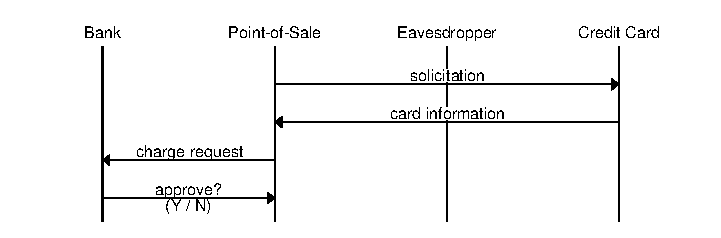
\includegraphics{img/attack-3-eavesdrop.eps}
  \label{fig:insecure-eavesdropper}
\end{figure}

We have demonstrated the feasibility of this attack by building a very low form-factor antenna capable of eavesdropping on NFC communications.
Similar to the device described in \cite{kortvedt2009eavesdropping}, we modified a MIFARE NFC tag to act as an antenna by disabling the chip at the center and attaching leads to either side of the coil where they connect to the chip.
We then measure the voltage induced in the coil.

In Figure \ref{fig:insecure-eavesdropper-antenna}, we show our NFC eavesdropping antenna next to a credit card for scale.
The resulting antenna is paper thin, flexible, approximately 3cm in diameter and adhesive on one side.
As such, it can easily be concealed within range of a Point of Sale.

\begin{figure}
  \caption{Eavesdropping Antenna (credit card for scale)}
  \centering
    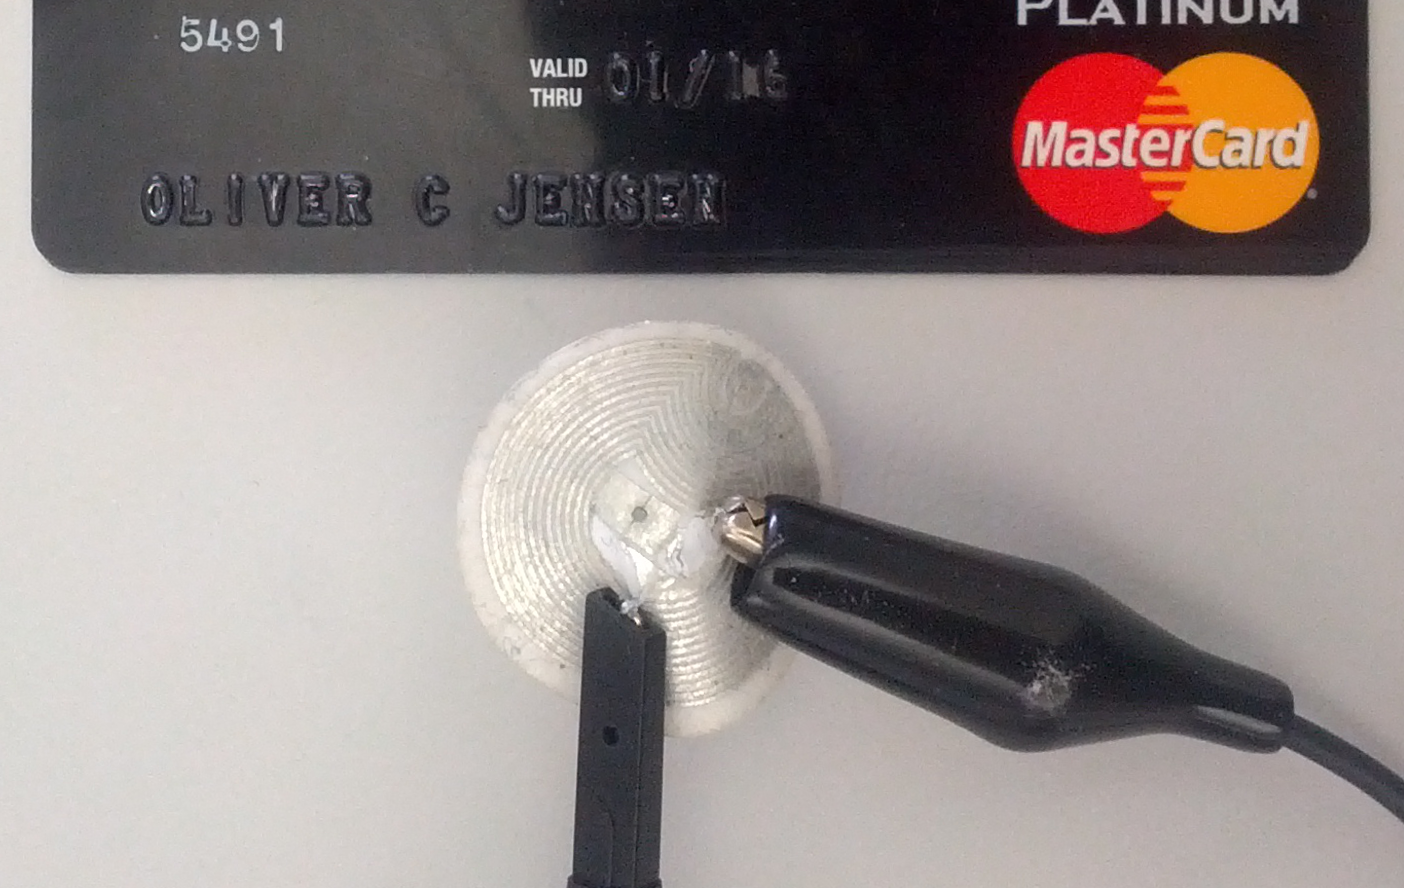
\includegraphics[width=1.0\textwidth, clip=true, trim=0 0 0 0]{img/attack-3-eavesdrop-photo.png}
  \label{fig:insecure-eavesdropper-antenna}
\end{figure}

By connecting such a makeshift antenna to a software-defined radio (available very inexpensively online) and recording the captured signal with a program like GNU Radio, an eavesdropper can record all transmissions that occur between the Point of Sale and credit cards.
We have written a simple program to read these signal-recordings and decode the messages in each direction.

In the Insecure CC Protocol, an eavesdropper acquires the credit card number, expiration date and the issuing bank name.
(The eavesdropper also acquires the iCVV, but since this is used immediately in the current transaction, the acquired iCVV is of no value.)





\subsection{Skimming}
\label{sec:insecure-skimmer}
The goal of a skimmer is to perform a purchase on behalf of the victim, without the victim's knowledge or consent.
First, the skimmer masquerades as a Point of Sale to the victim's credit card, acquiring the credit card number, expiration date, issuing bank name, and the next iCVV.
Subsequently, the skimmer masquerades as a credit card to a legitimate Point of Sale, making a purchase on behalf of the victim by replaying the skimmed credit card information and the iCVV.
An outline of this attack is shown in Figure~\ref{fig:insecure-skimmer}.

\begin{figure}
  \caption{Skimming -- FIX POS LABEL}
  \centering
    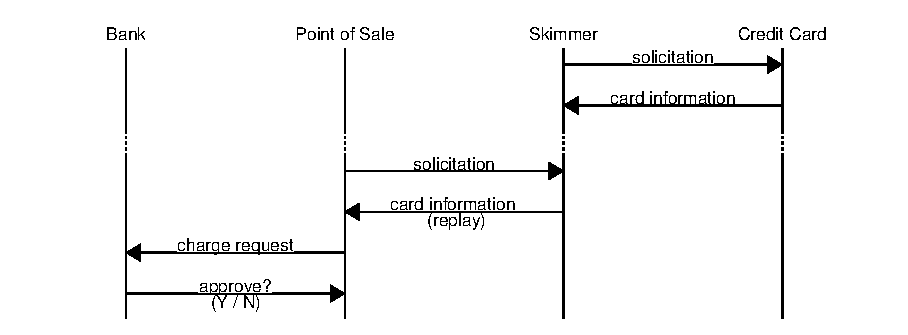
\includegraphics{img/attack-3-skim.eps}
  \label{fig:insecure-skimmer}
\end{figure}

This attack can be performed using a smart-phone with NFC capabilities.
An Android application called \emph{NFCProxy}\footnote{\emph{NFCProxy}\cite{NFCProxy}, presented at Defcon 20, can be downloaded here: \url{http://sourceforge.net/projects/nfcproxy/}} automates this attack, and is freely available online.
While \emph{NFCProxy} is not listed in the Google Play store, it can be downloaded from SourceForge and installed on the phone in a matter of minutes.

With \emph{NFCProxy} running, the skimmer brings his phone briefly within range of an NFC credit card to acquire the credit card information and  the iCVV.
When the skimmer wishes to perform the illegitimate purchase on behalf of the victim, the skimmer moves their phone within range of a Point of Sale as though it were a credit card.

In the Insecure CC Protocol, a skimmer may perform a single purchase (limited by the lack of subsequent iCVVs).
The skimmer must take care to perform this purchase before the credit card holder makes a purchase of their own, as this would invalidate the skimmed iCVV.
(The skimmer also gains all information that an eavesdropper would learn.)






\subsubsection{Relay Attacks}
\label{sec:insecure-relay}

Much like the skimmer, the goal of the relay attacker is to perform purchases on behalf of the victim, without the victim's knowledge or consent.
Multiple devices may be used to relay skimmed credit card information across a separate channel, effectively breaking down the assumption of proximity built into NFC.
This attack can also be performed using the \emph{NFCProxy} Android application, described in Section \ref{sec:insecure-skimmer}.
An outline of this attack is shown in Figure \ref{fig:insecure-relay}.

\begin{figure}
  \caption{Relay Attack FIX POS LABEL}
  \centering
    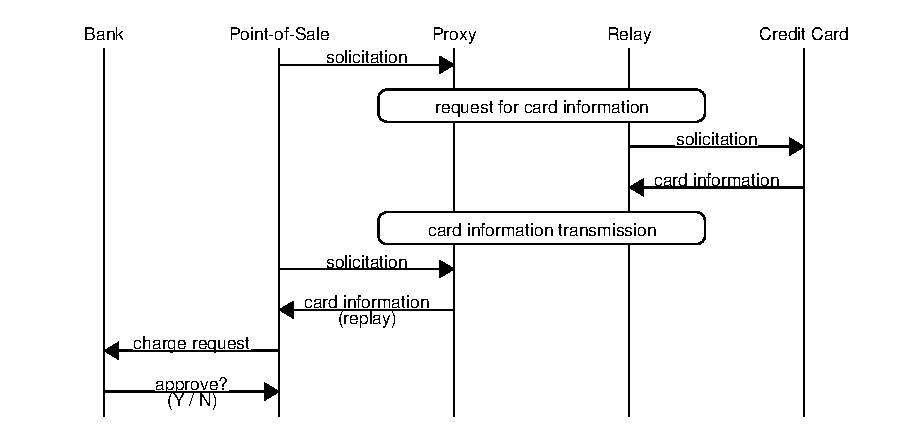
\includegraphics{img/attack-3-relay.eps}
  \label{fig:insecure-relay}
\end{figure}

In implementation, a relay attack is very similar to a skimming attack, with the exception that the skimmer is separated into two entities, called ``proxy'' and ``relay''.
These two entities are spatially disparate, but are connected through an out-of-band communication channel.
The relay positions his phone near the victim's credit card, while the proxy approaches a Point of Sale.
Whenever the proxy is ready to make a purchase, it sends a message to the relay requesting fresh values from the victim's credit card.

The relay skims the credit card, and forwards the card's information back to the proxy, enabling it to make a purchase on behalf of the victim.
These messages may be transmitted over any communication channel, but are most easily sent over a wireless LAN.

In the Insecure CC Protocol, a proxy may perform multiple purchases if the relay remains in proximity of the victim's credit card, querying it for fresh iCVVs for every purchase.





\subsubsection{Attacks Facilitated by Compromised Points of Sale}
\label{sec:insecure-compromised}

The Insecure CC Protocol implicitly trusts the ability of a Retailer to keep its data secure.
By allowing persistent sensitive information (e.g. the credit card number and expiration date) to be transmitted to a device under the Retailer's control,
  this protocol invites attacks on the Retailer's own systems.
We use this category of attacks to refer to any attacks which involve the Point of Sale or merchant performing (possibly unintentional) actions leading to credit card theft\footnote{
	In the Compromised Point of Sale model we consider only devices which correctly adhere to the protocol.
	We explicitly exclude what we term \emph{malicious} Points of Sale, those which may perform arbitrary actions such as refusing to randomize random values, etc.
	Defending against a malicious Point of Sale in any payment setting is much more involved, and is discussed later.
}.
For example, a Point of Sale might be compromised and re-programmed to transmit credit card information to an attacker after every successful purchase.
An outline of this attack is shown in Figure~\ref{fig:insecure-compromised}.

\begin{figure}[h!]
  \caption{Compromised Point of Sale}
  \centering
    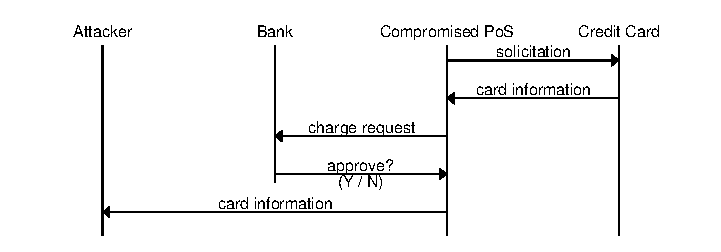
\includegraphics{img/attack-3-comppos.eps}
  \label{fig:insecure-compromised}
\end{figure}

The compromise of Points of Sale is far from a theoretical threat:
these attacks have become alarmingly commonplace, to the point that they have been covered by mainstream news sources including the New York Times \cite{neimanmarcushack} and the Wall Street Journal \cite{targethack}\cite{homedepothack}.

In November through December 2013, unauthorized access was gained to an estimated 40,000 Points of Sale used by U.S. retailer Target.
This data breach was widely publicized, as it resulted in the compromise of \emph{40 million} credit and debit cards, and other personal information of 70 million customers as reported in the Wall Street Journal \cite{targethack}.

More recently, in September 2014, Home Depot confirmed a similar data breach.
According to subsequent investigations, it appears that the same malware as was used against Target was at the heart of the Home Depot breach.
During this breach, attackers stole \emph{56 million} credit and debit cards, also as reported in the Wall Street Journal \cite{homedepothack}.

Other recent victims of Compromised Points of Sale include other retailers
	(e.g. Neiman Marcus in July through October of 2013, in which attackers stole an estimated 1.1 million credit and debit cards)\cite{neimanmarcushack},
	grocery stores (e.g. Supervalu in June through July of 2014, in which it is estimated that attackers stole ``millions'' of credit and debit cards\cite{supervaluhack}),
	as well as restaurants (e.g. P.F. Chang's in September 2013 through June 2014, in which attackers stole an estimated 7 million credit and debit cards\cite{pfchanghack}).

Since 2014, headlines regarding data theft from compromised Points of Sale have diminished,
    not because the attacks have slowed, but because they have become so prevalent they are no longer headline-worthy.
